% All revision tables and Fig. 2 in one document. Build:
%   tectonic reports/pilot_stability/paper/revision_tables.tex
\documentclass[10pt]{article}
\usepackage[a4paper,landscape,margin=1.6cm]{geometry}
\usepackage{booktabs}
\usepackage{graphicx}
\usepackage[T1]{fontenc}
\usepackage{lmodern}
\usepackage{textcomp}
\usepackage{newunicodechar}
\newunicodechar{−}{$-$}
\newunicodechar{×}{$\times$}
\newunicodechar{–}{--}
\newunicodechar{≥}{$\geq$}
\setlength{\parindent}{0pt}
\title{RAGFailBench revision: tables and figure}
\date{}
\begin{document}
\maketitle
\section*{Model evaluation (Tables XII, XIII, XV, XVI)}
\begin{table*}[t]
\centering
\caption{Score by condition, mean $\pm$ std over three seeded runs. Score is answer accuracy for answer-expected conditions (conflict: handled rate) and correct-abstention rate for abstain-expected ones; closed-book is accuracy with no context (prior knowledge, a probe outside FRS). $\Delta$ is the paired drop in percentage points against each item's own parent clean seed; FRS = 1 $-$ mean paired drop.}
\small
\begin{tabular}{llll}
\toprule
Condition & nova-pro score ($\Delta$ pp) & llama score ($\Delta$ pp) & gpt-oss score ($\Delta$ pp) \\
\midrule
clean & 0.97 $\pm$ 0.01 & 0.98 $\pm$ 0.01 & 0.97 $\pm$ 0.00 \\
missing\_evidence (abstain) & 0.94 $\pm$ 0.00 (-6.3) & 0.95 $\pm$ 0.00 (-5.2) & 0.93 $\pm$ 0.00 (-6.6) \\
hard\_negative (abstain) & 0.96 $\pm$ 0.01 (-4.2) & 0.96 $\pm$ 0.01 (-4.5) & 0.96 $\pm$ 0.00 (-4.5) \\
conflict & 0.74 $\pm$ 0.03 (-23.4) & 0.75 $\pm$ 0.01 (-23.3) & 0.65 $\pm$ 0.01 (-32.1) \\
context\_noise & 0.97 $\pm$ 0.01 (-0.3) & 0.98 $\pm$ 0.00 (+0.0) & 0.97 $\pm$ 0.00 (-0.4) \\
chunk\_boundary & 0.95 $\pm$ 0.01 (-1.5) & 0.97 $\pm$ 0.01 (-0.9) & 0.93 $\pm$ 0.01 (-4.4) \\
evidence\_position & 0.97 $\pm$ 0.01 (-0.5) & 0.98 $\pm$ 0.01 (+0.2) & 0.97 $\pm$ 0.01 (-0.1) \\
closed-book (probe) & 0.30 $\pm$ 0.03 & 0.47 $\pm$ 0.01 & 0.48 $\pm$ 0.03 \\
FRS & 0.940 $\pm$ 0.005 & 0.944 $\pm$ 0.002 & 0.920 $\pm$ 0.003 \\
\bottomrule
\end{tabular}
\end{table*}

\begin{table*}[t]
\centering
\caption{Abstention / answered-correctly / hallucination rate by condition, mean $\pm$ std over three seeded runs. For abstain-expected operators a non-abstention is either correct (prior knowledge or a residual partial leak) or a hallucination (wrong answer).}
\small
\begin{tabular}{llll}
\toprule
Condition & nova-pro abst. / ans.-correct / halluc. & llama abst. / ans.-correct / halluc. & gpt-oss abst. / ans.-correct / halluc. \\
\midrule
missing\_evidence & 0.94 $\pm$ 0.00 / 0.01 $\pm$ 0.00 / 0.06 $\pm$ 0.01 & 0.95 $\pm$ 0.00 / 0.01 $\pm$ 0.00 / 0.04 $\pm$ 0.00 & 0.93 $\pm$ 0.00 / 0.02 $\pm$ 0.00 / 0.05 $\pm$ 0.00 \\
hard\_negative & 0.96 $\pm$ 0.01 / 0.00 $\pm$ 0.00 / 0.04 $\pm$ 0.01 & 0.96 $\pm$ 0.01 / 0.01 $\pm$ 0.00 / 0.04 $\pm$ 0.01 & 0.96 $\pm$ 0.00 / 0.01 $\pm$ 0.00 / 0.04 $\pm$ 0.00 \\
conflict & 0.00 $\pm$ 0.00 / — / 0.25 $\pm$ 0.03 & 0.01 $\pm$ 0.01 / — / 0.24 $\pm$ 0.01 & 0.01 $\pm$ 0.00 / — / 0.33 $\pm$ 0.01 \\
context\_noise & 0.00 $\pm$ 0.00 / — / 0.01 $\pm$ 0.01 & 0.00 $\pm$ 0.00 / — / 0.01 $\pm$ 0.01 & 0.00 $\pm$ 0.00 / — / 0.01 $\pm$ 0.00 \\
chunk\_boundary & 0.01 $\pm$ 0.00 / — / 0.02 $\pm$ 0.01 & 0.01 $\pm$ 0.01 / — / 0.00 $\pm$ 0.00 & 0.04 $\pm$ 0.01 / — / 0.01 $\pm$ 0.00 \\
evidence\_position & 0.00 $\pm$ 0.00 / — / 0.01 $\pm$ 0.01 & 0.00 $\pm$ 0.00 / — / 0.00 $\pm$ 0.00 & 0.00 $\pm$ 0.00 / — / 0.01 $\pm$ 0.00 \\
\bottomrule
\end{tabular}
\end{table*}

\begin{table*}[t]
\centering
\caption{Paired drop (pp) by severity: mean $\pm$ std over three seeded runs of the three-model mean. For abstain-expected operators the drop is the rate of failing to abstain; missing\_evidence severity is closeness of the remaining context to the removed evidence.}
\small
\begin{tabular}{llll}
\toprule
Operator & low & medium & high \\
\midrule
missing\_evidence & 0.2 $\pm$ 0.2 & 5.7 $\pm$ 0.3 & 13.2 $\pm$ 1.1 \\
hard\_negative & 3.2 $\pm$ 0.7 & 4.1 $\pm$ 0.5 & 5.8 $\pm$ 1.4 \\
conflict & 9.7 $\pm$ 1.5 & 27.0 $\pm$ 1.2 & 42.0 $\pm$ 0.3 \\
context\_noise & -0.1 $\pm$ 0.3 & 0.3 $\pm$ 0.3 & 0.5 $\pm$ 0.3 \\
chunk\_boundary & -0.1 $\pm$ 0.6 & 2.1 $\pm$ 1.2 & 5.4 $\pm$ 1.0 \\
evidence\_position & 0.2 $\pm$ 0.3 & 0.1 $\pm$ 0.6 & 0.1 $\pm$ 0.5 \\
\bottomrule
\end{tabular}
\end{table*}

\begin{table*}[t]
\centering
\caption{Conflict outcomes, mean $\pm$ std (\%) over three seeded runs. Handled = gold, both values, or an acknowledged conflict. Aware = prompt that permits flagging a conflict (probe, excluded from FRS). Prior known/unknown splits by closed-book correctness.}
\small
\begin{tabular}{llllllllll}
\toprule
Model & Prompt & Gold \% & Alternate \% & Both \% & Acknowledged \% & Handled \% & Judge-only \% & Handled, prior known \% & Handled, prior unknown \% \\
\midrule
nova-pro & default & 62.4 $\pm$ 2.5 & 23.0 $\pm$ 1.9 & 11.2 $\pm$ 0.3 & 11.3 $\pm$ 0.5 & 73.6 $\pm$ 2.5 & 72.0 $\pm$ 2.4 & 85.0 $\pm$ 1.7 & 68.9 $\pm$ 3.6 \\
nova-pro & aware & 33.8 $\pm$ 2.3 & 10.6 $\pm$ 0.8 & 52.1 $\pm$ 3.1 & 54.2 $\pm$ 2.7 & 87.4 $\pm$ 1.1 & 39.2 $\pm$ 3.2 & 91.8 $\pm$ 2.9 & 85.5 $\pm$ 0.3 \\
llama & default & 37.1 $\pm$ 3.7 & 17.6 $\pm$ 1.3 & 36.8 $\pm$ 3.9 & 37.6 $\pm$ 4.0 & 74.6 $\pm$ 0.9 & 60.9 $\pm$ 1.7 & 79.3 $\pm$ 2.2 & 70.3 $\pm$ 2.1 \\
llama & aware & 17.0 $\pm$ 2.1 & 3.1 $\pm$ 0.1 & 74.1 $\pm$ 2.3 & 80.1 $\pm$ 1.8 & 94.9 $\pm$ 0.1 & 32.9 $\pm$ 2.8 & 96.4 $\pm$ 0.4 & 93.6 $\pm$ 0.5 \\
gpt-oss & default & 51.6 $\pm$ 2.0 & 27.9 $\pm$ 1.3 & 13.8 $\pm$ 1.9 & 13.9 $\pm$ 2.0 & 65.4 $\pm$ 0.7 & 62.6 $\pm$ 0.2 & 74.6 $\pm$ 2.1 & 57.2 $\pm$ 1.4 \\
gpt-oss & aware & 14.7 $\pm$ 2.2 & 3.4 $\pm$ 0.3 & 72.1 $\pm$ 2.9 & 84.1 $\pm$ 2.6 & 95.0 $\pm$ 0.5 & 23.7 $\pm$ 1.0 & 95.6 $\pm$ 2.2 & 94.3 $\pm$ 1.1 \\
\bottomrule
\end{tabular}
\end{table*}

\clearpage
\section*{Confidence intervals, McNemar tests, correctness signals (Tables XVII, XIX)}
\begin{table}[t]
\centering\small
\caption{Paired drop (pp) and FRS with 95% CIs, pooled over three seeded runs; cluster bootstrap over 600 parent clean seeds, 2000 resamples.}
\begin{tabular}{lccc}
\toprule
Condition & nova-pro & llama & gpt-oss \\
\midrule
missing\_evidence & 6.3 [5.1, 7.7] & 5.2 [4.1, 6.5] & 6.6 [5.3, 8.0] \\
hard\_negative & 4.2 [2.9, 5.6] & 4.5 [3.1, 5.9] & 4.5 [3.2, 5.9] \\
conflict & 23.4 [20.6, 25.9] & 23.3 [20.7, 25.8] & 32.1 [29.4, 34.7] \\
context\_noise & 0.3 [-0.8, 1.4] & 0.0 [-0.7, 0.7] & 0.4 [-0.3, 1.2] \\
chunk\_boundary & 1.5 [0.3, 2.8] & 0.9 [-0.3, 2.1] & 4.4 [2.9, 5.9] \\
evidence\_position & 0.5 [-0.5, 1.6] & -0.2 [-1.1, 0.6] & 0.1 [-0.8, 0.9] \\
FRS & 0.940 [0.932, 0.948] & 0.944 [0.937, 0.951] & 0.920 [0.912, 0.928] \\
\bottomrule
\end{tabular}
\end{table}

\begin{table}[t]
\centering\small
\caption{FRS difference between models with paired 95% CIs (same resampled seeds), pooled over three seeded runs; cluster bootstrap over 600 parent clean seeds, 2000 resamples.}
\begin{tabular}{lcc}
\toprule
Models & ΔFRS [95% CI] & CI excludes 0 \\
\midrule
nova-pro -- llama & -0.004 [-0.014, +0.006] & no \\
nova-pro -- gpt-oss & +0.020 [+0.009, +0.030] & yes \\
llama -- gpt-oss & +0.024 [+0.015, +0.033] & yes \\
\bottomrule
\end{tabular}
\end{table}

\clearpage
\section*{Human audit (Tables V, VI, VIII, IX, XI human rows)}
\begin{table*}[t]
\centering
\caption{Human audit summary (replaces the HAR and failure-validity rows of Table V). Blind stratified sample from the three seeded runs; 95\% Wilson CIs. Annotator 1 is primary.}
\small
\begin{tabular}{p{0.36\textwidth}ll}
\toprule
Metric & Annotator 1 & Annotator 2 \\
\midrule
Human acceptance (HAR), clean seeds & 84.0\% {[}71.5, 91.7{]} (42/50) & 86.0\% {[}73.8, 93.0{]} (43/50) \\
Failure injection valid & 96.3\% {[}87.5, 99.0{]} (52/54) & 98.1\% {[}90.2, 99.7{]} (53/54) \\
Failure label (answer available) correct & 100.0\% {[}93.4, 100.0{]} (54/54) & 100.0\% {[}93.4, 100.0{]} (54/54) \\
\bottomrule
\end{tabular}
\end{table*}

\begin{table*}[t]
\centering
\caption{Human audit per seeded run (replaces Tables VI and VIII human columns): clean seeds kept and failure cases judged valid, per annotator. Per-run samples are small (16–17 seeds, 18 failure cases); pooled values are in the summary table.}
\small
\begin{tabular}{lllll}
\toprule
Run & HAR A1 & HAR A2 & Failure validity A1 & Failure validity A2 \\
\midrule
pilot\_stability\_s42 & 16/16 & 16/16 & 17/18 & 17/18 \\
pilot\_stability\_s123 & 13/17 & 13/17 & 17/18 & 18/18 \\
pilot\_stability\_s2026 & 13/17 & 14/17 & 18/18 & 18/18 \\
All runs & 42/50 & 43/50 & 52/54 & 53/54 \\
\bottomrule
\end{tabular}
\end{table*}

\begin{table*}[t]
\centering
\caption{Primary reason for the 8 of 50 audited clean seeds annotator 1 did not keep (replaces Table IX). One primary reason per row from the structured flags, in the order listed; the free-text note gives the detail.}
\small
\begin{tabular}{p{0.25\textwidth}llp{0.14\textwidth}p{0.3\textwidth}}
\toprule
Reason & Count & Percent & Structured basis & Rows \\
\midrule
Time-sensitive phrasing & 2 & 25.0\% & time\_sensitive\_ok = no & C022 (fix), C027 (fix) \\
Answer not unique & 1 & 12.5\% & answer\_unique = no & C002 (fix) \\
Unclear question (reference, premise, wording) & 4 & 50.0\% & question\_clear = no & C010 (fix), C039 (fix), C044 (fix), C047 (fix) \\
Other (trivial; see note) & 1 & 12.5\% & no flag set & C040 (reject) \\
\bottomrule
\end{tabular}
\end{table*}

\begin{table*}[t]
\centering
\caption{Failure-injection verification: automatic check on every case versus the human audit (replaces Table XI). Per-operator samples are 9 cases (3 per severity).}
\small
\begin{tabular}{p{0.36\textwidth}ll}
\toprule
Check & Annotator 1 & Annotator 2 \\
\midrule
Automatic structural verification (leakage / label check), all cases & 94.9\% $\pm$ 0.3\% pass &  \\
Human: injection valid, all operators & 96.3\% {[}87.5, 99.0{]} (52/54) & 98.1\% {[}90.2, 99.7{]} (53/54) \\
  missing\_evidence & 9/9 & 9/9 \\
  hard\_negative & 9/9 & 9/9 \\
  conflict & 7/9 & 8/9 \\
  context\_noise & 9/9 & 9/9 \\
  chunk\_boundary & 9/9 & 9/9 \\
  evidence\_position & 9/9 & 9/9 \\
\bottomrule
\end{tabular}
\end{table*}

\begin{table*}[t]
\centering
\caption{Inter-annotator agreement on the same audit rows. The second annotator had seen the first annotator's labels in an earlier pass, so agreement may be overstated. Kappa is undefined when both annotators used a single identical label.}
\small
\begin{tabular}{llll}
\toprule
Field & n & Agreement & Cohen's kappa \\
\midrule
decision & 50 & 98.0\% & 0.92 \\
question\_clear & 50 & 98.0\% & 0.85 \\
answer\_in\_evidence & 50 & 100.0\% & undefined (one label only) \\
answer\_unique & 50 & 98.0\% & 0.66 \\
time\_sensitive\_ok & 50 & 100.0\% & 1.00 \\
needs\_title & 50 & 100.0\% & 1.00 \\
human\_injection\_valid & 54 & 98.1\% & 0.66 \\
human\_label\_correct & 54 & 100.0\% & undefined (one label only) \\
severity\_ok & 54 & 74.1\% & 0.14 \\
\bottomrule
\end{tabular}
\end{table*}

\clearpage
\begin{figure}[t]
\centering
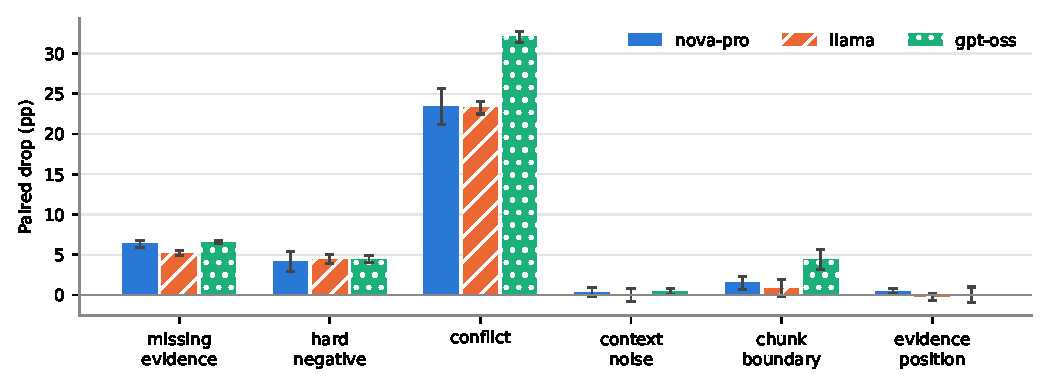
\includegraphics[width=0.75\linewidth]{fig2_paired_drop.pdf}
\caption{Paired performance drop by failure operator (Fig. 2).}
\end{figure}
\end{document}
